% -*- LaTeX -*- This is LaTeX2e code

\section{Nearest Neighbor Problems}\label{sec:nn}

\subsection{Closest Pair}

Given a set $P$ of $n$ points in the plane stored in an array \texttt{A}$[0
\ldots n - 1]$, a closest pair is a pair of points in $P$ whose Euclidean
distance is smallest among all pairs of points. We modify an algorithm by
Bentley and Shamos~\cite{bentley:divide-and-conquer} to compute the closest
pair in \Oh{n \log n} time using only \Oh{1} extra space.

Algorithm~\ref{alg:bentley} describes a slightly modified version of Bentley's
divide-and-conquer algorithm for finding the closest pair.  The algorithm
works by drawing an imaginary vertical dividing line through the median
$X$-coordinate.  The algorithm then finds the closest pair with both points to
the left of this line, the closest pair with both points to the right of this
line and then finds the closest pair with one point on the left and one point
on the right of the line.  The first two closest pairs are computed with
recursive calls while the third closest pair is accomplished by a vertical
plane sweep of all the points that are ``close to'' the dividing line.
 
\begin{algorithm} \label{alg:nn}
  \caption{$\textsc{Nearest-Neighbor}(A,b,e)$: Divide-and-Conquer algorithm for finding a closest
    pair~\cite{bentley:divide-and-conquer}.} 
  \begin{algorithmic}[1]
    \REQUIRE All points in the input array $A$ are sorted according to
    $Y$-coordinate.
    \ENSURE The first two points in the array $A[b,\ldots,e-1]$ realize the closest pair and the remaining points are sorted by $Y$-coordinate.
    \IF{$e-b < 16$} 
      \STATE Compute a closest pair using a brute-force
algorithm, stably place them at the front of the current subarray and return.
    \ELSE
      \STATE Compute the median $X$-coordinate $x$ using
Algorithm~\ref{alg:selectk} (\textsc{Select}) while maintaining the array
sorted by $Y$-coordinate.
      \STATE Using Algorithm~\ref{alg:sortedSubsetSelection}, stably select all
elements of $A[b,\ldots,e-1]$ with $x$ coordinate less than or equal $x$ so
that they are stored in $A[b,\ldots,\lfloor e/2\rfloor-1]$. 
      \STATE \textsc{Nearest-Neighbor}($A,b,\lfloor e/2 \rfloor$)
      \STATE Using Algorithm~\ref{alg:revertSortedSubsetSelection}, restore
$A[b,\ldots,e-1]$ so that it is sorted by $Y$ coordinate.  Stably store the
closest pair from the previous step in $A[b]$ and $A[b+1]$.
       \STATE Using Algorithm~\ref{alg:sortedSubsetSelection}, stably select all elements of $A[b,\ldots,e-1]$ with $x$
coordinate greater than $x$ so that they are stored in
$A[\lfloor e/2\rfloor,\ldots,e-1]$. 
      \STATE \textsc{Nearest-Neighbor}($A,\lfloor e/2 \rfloor$,e)
       \STATE Using Algorithm~\ref{alg:revertSortedSubsetSelection}, restore
$A[b,\ldots,e-1]$ so that it is sorted by $Y$ coordinate.  Stably store the
closest pair from Step~6 or the closest pair from the previous step (whichever
is closer) at
locations $A[b]$ and $A[b+1]$.
      \STATE Let $\delta$ be the distance between $A[b]$ and $A[b+1]$.
      \STATE Using Algorithm~\ref{alg:sortedSubsetSelection}, extract in $Y$-sorted order the points of $A[b,\ldots,e-1]$ that fall within a
                strip of width $2\delta$ centered at the median $X$-coordinate of $A[b,\ldots,e-1]$.
         \STATE Scan the points in this strip to determine whether there is a pair of
                points with distance smaller than $\delta$. Update $\delta$ and
                the closest pair as necessary. 
        \STATE Using Algorithm~\ref{alg:revertSortedSubsetSelection}, restore
$A[b,\ldots,e-1]$ so that it is sorted by $Y$ coordinate.  Stably store the closest pair 
at
locations $A[b]$ and $A[b+1]$.
    \ENDIF
  \end{algorithmic}
\end{algorithm}

Note that the recursion tree for Bently and Shamos' algorithm is balanced
with the the two recursive calls occuring in lines 6 and 9 and that this
algorithm fits into the framework of the Algorithm~\ref{stackless}
(\textsc{Stackless-Recursive}).  In particular, PROCESS~1 takes place in
line~2, PROCESS~3 takes place in lines 


. For
simplicity of exposition, we stopped the recursion when an instance of size at
most 16 is reached.  Therefore, to apply our space-efficient recursion
template, we first need to show how to compute the base instances (i.e. leaves
of the recursion tree) and then elaborate on some of the details within the
PROCESSES.  The base of the recusion is trivially computed by running any
\emph{in-place} sorting algorithm, e.g., \emph{heapsort}~\cite{floyd:245}, to
sort the points according to their $X$-coordinate in \Oh{n \log n} time using
\Oh{1} extra space.

Now, to elaborate on the PROCESSES. First, steps in PROCESS 1 can be trivially
completed in \Oh{1} time and space since the instances are of size at most 16.
The steps in PROCESS 2 do not need to be computed since we are pre-computing
the base instances.  Next, we show how to space-efficiently perform the steps
in PROCESS 3. The two subarrays being processed are $A[b,\ldots,\lfloor e/2
\rfloor-1]$ and $A[\lfloor e/2 \rfloor + 1,\ldots, e-1]$. We first need to
determine the minimal $\delta$ given by the two locally closest pairs. This is
easy since the invariant maintained is that the locally closest pair is stored
in the first two positions of each of the two subarrays, i.e.
$A[b,\ldots,b+1]$ and $A[\lfloor e/2 \rfloor + 1, \lfloor e/2 \rfloor + 2]$,
and the remaining elements in each of the two sub-arrays are sorted by
$Y$-coordinate. We record the pair of points forming the minimal $\delta$ in
extra memory. Before moving on to the merge step, we compute and record in
extra memory the point with maximum $X$-coordinate in $A[b,\ldots, \lfloor e/2
\rfloor-1]$ and re-order the two sub-arrays such that each of them is sorted
by $Y$-coordinate.  Thus, the steps in PROCESS 3 can be accomplished in \Oh{n}
time using \Oh{1} extra space.

For the merge step, we need to merge two lists sorted by $Y$-coordinate into
one list sorted by $Y$-coordinate. It is well known that this can be achieved
in \Oh{n} time with the use of two pointers which is \Oh{1} extra space.  We
now proceed to the three steps in PROCESS 4. 

The first step is to extract the points that
fall within a strip of width $2\delta$ centered at the median $X$-coordinate of $A[b,\ldots,e-1]$. 
Note that the point with median $X$-coordinate in $A[b,\ldots,e-1]$ is simply the point with 
maximum $X$-coordinate in $A[b,\ldots,\lfloor e/2 \rfloor]$, which we pre-computed prior to the merge.
With this median $X$-coordinate, we use SortedSubsetSelection on $A[b,\ldots,e-1]$
to select all of the points that fall within the $2\delta$ strip. Let $A[b,\ldots,m-1]$ contain the
points falling in the strip. Note that these points are sorted by $Y$-coordinate.

The second step is simple since the points falling in the $2\delta$ strip are sorted by $Y$-coordinate and the standard scan as described in 
Bentley and Shamos can be applied. Essentially, for each point $A[i]$, Bentley and Shamos showed that if there is a pair of points
whose distance is less than $\delta$, it can only be formed with the 7 points following it in $Y$-sorted order (i.e. $A[i+1] \ldots A[i+7]$).
Once the scan is complete, the closest pair in $A[b,\ldots,e-1]$ is known and stored in extra memory.
Now, we undo the SortedSubsetSelection step since we know the values $b$, $m$ and $e$, which returns the array
in $Y$-sorted order as required. Thus, the second step uses \Oh{n} time and \Oh{1} extra space.

Finally, for the third step, in \Oh{n} time we stably place the pair of points forming the closest pair to the front of the array.
Since all the base instances can be computed in \Oh{n \log n} time and \Oh{1} extra space and each of the PROCESSES can be computed in
\Oh{n} time with \Oh{1} extra space, we conclude with the following:


\begin{theorem}
  Given a set $P$ of $n$ points in the plan stored in an array
  \texttt{A}$[0 \ldots n-1]$, a closest pair in $P$ can be computed in
  \Oh{n \log n} time using \Oh{1} extra memory.
\end{theorem}


\subsection{Bichromatic Closest Pair}

In the Bichromatic Closest Pair Problem, we are given a set $R$ of red
points and a set $B$ of blue points in the plane. The problem is to
return a pair of points, one red and one blue, whose distance is
minimum over all red-blue pairs. We assume that there are a total of $n$ points, with $m>0$ Blue points and $n-m+1>0$ Red points.
The input is given to us in an array $A[0,n-1]$ with each point being identified as either red or blue.

The solution is similar to the solution presented in the previous subsection, with a few subtle differences.
Prior to providing the solution to the whole problem, we first consider a special case  that is essential to 
the final solution and that highlights the main difference between the two problems. Assume that the red and blue sets are
separated by a vertical line, with the red points on the left of the line
and the blue points on the right of the line. The solution to this problem is similar to
the merge step in the previous section, except that we no longer have
the luxury of the value $\delta$ to restrict our search. To circumvent this problem we
proceed in the following way. 

\begin{algorithm}
  \caption{Bi-Chromatic-Closest-Vertically-Separated-Pair($R,B,\ell$): Bichromatic closest pair when $R$ and $B$ are separated by
    a vertical line $\ell$ and $R$ is to the left of $\ell$.} 
  \label{alg:bichromatic-separated}
  \begin{algorithmic}[1]
    \REQUIRE All points in $R[0,n-1]$ and $B[0,m-1]$ are sorted by
    $Y$-coordinate.  
    \ENSURE All points in $R$ and $B$ are sorted by
    $Y$-coordinate, and the bichromatic closest pair is reported.
    \STATE Let $N=n$ the size of $|R|$ and let $M=m$ the size of $|B|$.
    \WHILE{$n>16$ or $m>16$}
        \STATE Assume $n\geq m$, otherwise reverse the roles of $R$ and $B$.
        \STATE Pick a random element $r$ from $R[0,n-1]$.
        \STATE Find an element $b \in B[0,m-1]$ closest to $r$.
        \STATE Compute the left envelope of disks having radius
               $\text{dist}(r,b)$ centered at each of the points in $B[0,m-1]$.
        \IF{less than $n/2$ elements of $R[0,n-1]$ are to the left of envelope}
               \STATE undo the envelope computation and repeat the last 3 steps.
        \ELSE
               \STATE Move exactly $\lfloor n/2\rfloor$ elements from $R[0,n-1]$ that are to the left of the blue 
                      envelope into $R[0,\lfloor n/2 \rfloor +1]$. 
               \STATE Store $2(n/2 - \lfloor n/2 \rfloor)$ on stack $S$.
               \STATE Store 1 bit on stack $S$ when $n \geq m$ and 0 bit otherwise.
               \STATE Undo the envelope computation.
               \STATE Let $n := \lfloor n/2 \rfloor$.
        \ENDIF
    \ENDWHILE
    \STATE Compute and report a bichromatic closest pair using a brute-force algorithm since both $n$ and $m$ are less than 16.
    \STATE UNDO operations to restore $Y$-sorted order for both $R$ and $B$:
    \WHILE {$n < N$ or $m < M$}
         \STATE F := Pop top bit off stack.
         \STATE R := Pop top remainder off stack.
         \IF{$F$ is 1 (i.e. $n \geq m$)}
            \STATE $N_1 := 2n + R$. 
            \STATE UndoSubsetSelection($R,0,N_1,n$).
            \STATE $n := N_1$.
         \ELSE 
            \STATE \COMMENT{$F$ is 0 (i.e. $n < m$)}
            \STATE $M_1 := 2m + R$.
            \STATE UndoSubsetSelection($B,0,M_1,m$).
            \STATE $m := M_1$.
         \ENDIF
    \ENDWHILE
  \end{algorithmic}
\end{algorithm}

\begin{figure}
  \centerline{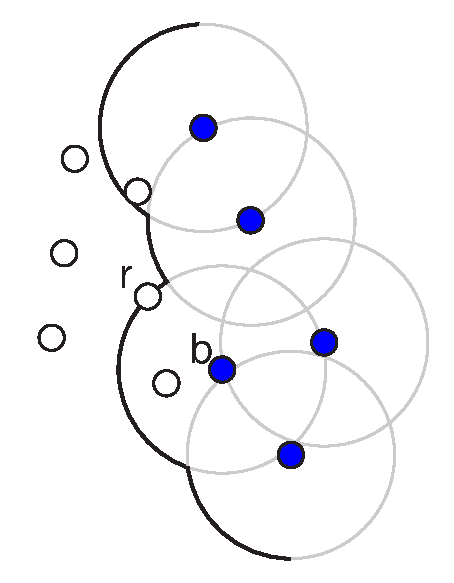
\includegraphics[height=5cm]{biclosest_algorithm}}
  \caption{Left envelope of disks centered at blue points (red
    points are drawn as hollow disks).}
  \label{fig:biclosest_algorithm}
\end{figure}

Algorithm \ref{alg:bichromatic-separated} runs in linear-expected time since
each time through the first while loop, with constant probability, we reduce
the size of $R$ or $B$ by a half.  This algorithm can be implemented using
only a constant amount of extra memory.  In the first while loop, there are
two steps we elaborate on: (1) how to compute and undo the left-envelope, and
(2) how to identify points to the left of the blue envelope. We begin with the
former.

Computing the left-envelope (portions of the disks visible
from the point $(-\infty, 0)$), is very similar to the convex hull
problem and can be solved in \Oh{n} time and \Oh{1} extra memory using an algorithm identical
to Graham's scan since the points are sorted by $Y$-coordinate.  The
implementation of Graham's scan given by Br\"onnimann
\etal~\cite{bronnimann:convex} achieves this with the output being an 
array that contains the elements that contribute to the left envelope
in the first part of the array sorted by $Y$-coordinate and the elements that do not contribute
in the second part of the array. Also, we observe that it is not
particulary difficult to run Graham's scan {\em in reverse} to restore
the $<_y$ sorted order of the elements in \Oh{n} time once we are done
with the left envelope. To see this, consider the following
pseudo-code implementation of Graham's Scan as outlined in \cite{bronnimann:convex}
(Algorithm~\ref{alg:leftHull}):

\begin{algorithm}
  \caption{Computing the left convex hull of a point set.}
  \label{alg:leftHull}
  \begin{algorithmic}[1]
    \REQUIRE All points in the input array $A[0\ldots n-1]$ are sorted according to
    $y$-coordinate.
    \FOR{$i:=0$ to $n-1$}
      \WHILE{$(h \geq 2)$ and 
        (($\texttt{A}[h-2], \texttt{A}[h-1], \texttt{A}[i]$) does not form a right turn)}
        \STATE Set $h:=h-1$.
      \ENDWHILE
      \STATE Swap $\texttt{A}[i]$ and $\texttt{A}[h]$.
      \STATE Set $h=h+1$.
    \ENDFOR
  \end{algorithmic}
\end{algorithm}

The effect of this algorithm can be reversed by
Algorithm~\ref{alg:revertLeftHull}:

\begin{algorithm}
  \caption{Restoring the $<_y$-order after computing the left
    envelope.}
  \label{alg:revertLeftHull}
  \begin{algorithmic}[1]
    \REQUIRE{Array $\texttt{A}[0\ldots h]$ contains the result of running
      Algorithm~\ref{alg:leftHull} on (the sorted) array
      $\texttt{A}[0\ldots n-1]$.}
    \STATE Set $q:=n-1$.
    \WHILE{$h\neq q$}
      \IF{$\texttt{A}[q] <_y \texttt{A}[h]$}
        \STATE Swap $\texttt{A}[h]$ and $\texttt{A}[q]$.
        \STATE Set $q:=q-1$.
        \IF{$\texttt{A}[q] <_y \texttt{A}[h-1]$}
          \STATE Set $h:=h-1$.
        \ENDIF
        \WHILE{($\texttt{A}[h] <_y \texttt{A}[h+1]$) and 
        (($\texttt{A}[h-2], \texttt{A}[h-1], \texttt{A}[i]$) form a right turn)}
          \STATE Set $h:=h+1$.
        \ENDWHILE
      \ELSE
        \STATE Set $h:=h+1$.
      \ENDIF
    \ENDWHILE
  \end{algorithmic}
\end{algorithm}

We now address the problem of determining the red points that are to the left of the blue envelope. To determine whether or not
a given red point $p$ is to the left of the blue envelope, we compute the intersection of a horizontal line through $p$ with the
envelope (see Figure \ref{fig:biclosest_algorithm}). If the intersection point is to the right of $p$ then $p$ is to the left of the envelope.
By scanning the red points from top to bottom and simultaneously scanning the blue envelope from top to bottom, similar to merging
of two sorted lists, all of these intersections can be computed in linear time. We select exactly $\lfloor n/2 \rfloor$ elements of $R$ 
to discard in order to simplify the undo step, similar to what was done in the selection problem.


We now outline how the whole algorithms comes together. We first present the algorithm in standard recursive form.

\begin{algorithm} 
  \caption{Algorithm Bi-Nearest-Neighbor($A,b,e$): Divide-and-Conquer algorithm for finding bi-chromatic closest
    pair.}\label{alg:binn}
  \begin{algorithmic}[1]

    \REQUIRE All points in the input array $A$ are sorted according to
    $X$-coordinate.

    \ENSURE First two points in the array $A[b,\ldots,e]$ realize the
    bi-chromatic closest pair provided $A[b,\ldots,e]$ contains at least
    one red and one blue point and the remaining points are sorted
    according to~$<_Y$.

    \IF{$e-b < 16$}
	 \STATE PROCESS 1: Sort the points according to $Y$-coordinate.
	 If there are at least one red and one blue points, compute
	 a bi-chromatic closest pair using a brute-force algorithm,
	 and stably place them at the front of the current subarray.
    \ELSE
         \STATE PROCESS 2: Stably partition the array based upon the median $X$-coordinate and recurse.
         \STATE Bi-Nearest-Neighbor($A,b,\ldots,\lfloor e/2 \rfloor$)
         \STATE Bi-Nearest-Neighbor($A,\lfloor e/2 \rfloor + 1, e$)
         \STATE PROCESS 3: Record the minimum bi-chromatic closest pair in each of the two subarrays.
         \STATE Let $R_l$ represent the red points in $A[b,\ldots,\lfloor e/2 \rfloor]$.
         \STATE Let $B_r$ represent the blue points in $A[\lfloor e/2 \rfloor + 1,\ldots,e]$.
         \IF{$R_l > 0$ and $B_r > 0$}
               \STATE Compute the Bi-chromatic closest pair for $R_l$ and $B_r$ separated by a line. 
         \ENDIF
         \STATE Let $B_l$ represent the blue points in $A[b,\ldots,\lfloor e/2 \rfloor]$.
         \STATE Let $R_r$ represent the red points in $A[\lfloor e/2 \rfloor + 1,\ldots,e]$.
         \IF{$B_l > 0$ and $R_r > 0$}
               \STATE Compute the Bi-chromatic closest pair for $B_l$ and $R_r$ separated by a line. 
         \ENDIF
         \STATE Compute the minimum of all the bi-chromatic closest pairs.
         \STATE Scan both subarrays such that all points are sorted according to~$<_y$.
         \STATE Stably place the bi-chromatic closest pair to the front of the array.
    \ENDIF
  \end{algorithmic}
\end{algorithm}

Note that this algorithm is similar to Algorithm \ref{alg:nn}. The only steps
we need to elaborate are the steps in PROCESS 3. Prior to Step 10, we use two
invocations to SortedSubsetSelection to move the red points in
$A[b,\ldots,\lfloor e/2 \rfloor]$ and blue points in $A[\lfloor e/2 \rfloor +
1, e]$ to the front of their respective arrays. We use Algorithm
\ref{alg:bichromatic-separated} to compute the closest red-blue pair.  We then
Undo this. Similarly, prior to Step 15, we use two invocations to
SortedSubsetSelection to move the blue points in $A[b,\ldots,\lfloor e/2
\rfloor]$ and red points in $A[\lfloor e/2 \rfloor + 1, e]$ to the front of
their respective arrays, use Algorithm \ref{alg:bichromatic-separated} to
compute the closest pair, followed by an Undo.  Since all the base instances
can be computed in \Oh{n \log n} time and \Oh{1} extra space and each of the
PROCESSES can be computed in \Oh{n} expected time with \Oh{1} extra space, we
conclude with the following:

\begin{theorem}
  Given sets $R$ and $B$ of \orderof{n} points in the plane, a closest
  bichromatic pair can be computed in \Oh{n \log n} expected time
  using \Oh{1} extra memory.
\end{theorem}

We note that if the points $R$ and $B$ are given in separate arrays as input, we can still achieve the same running time using \Oh{1} extra space albeit the 
details become much more tedious. Of course, using \Oh{\log n} extra space is trivial since Algorithm \ref{alg:binn} is in standard recursive form.
%
%\subsection{All Nearest Neighbors}\label{sec:allnn}
%
%In this section, we apply our divide-and-conquer scheme
%to solve the all-nearest neighbors problem space-efficiently. Again,
%we present a modification of Bentley and Shamos' algorithm.
%
%\begin{algorithm}
%  \caption{Divide-and-Conquer algorithm for computing all nearest
%    neighbors~\cite{bentley:divide-and-conquer}.}  
%  \begin{algorithmic}[1]
%    \REQUIRE All points in the input array $A$ are sorted according to
%    $x$-coordinate.
%    \ENSURE All points in $A$ are sorted according to~$<_y$, 
%    and for each point, its nearest neighbor in $A$ is known. 
%    \STATE  If $A$ stores only a constant number of points, sort the
%    points according to $<_y$, compute all nearest neighbors using 
%    a brute-force algorithm, and return.
%    \STATE  Subdivide the array based upon the median
%    $x$-coordinate $x=\ell$ and recurse on both subarrays $A_0$ and
%    $A_1$.  
%    \STATE  Simultaneously scan through both subarrays $A_0$ and $A_1$, and
%    for each point~$p\in A_i$ check all points in $A_{1-i}$ whose
%    nearest-neighbor ball contains the projection of $p$ onto the line
%    $x=\ell$. Update the nearest neighbor information as necessary.
%    \STATE  Merge the points according to $<_y$.
%  \end{algorithmic}
%\end{algorithm}
%
%We can make this algorithm space-efficient using the framework of
%Section 1. One detail, however, needs special attention: Bentley and
%Shamos argue that for each of the points in the sets to be merged,
%only ``a constant number other points needs be
%examined''~\cite[p.~229]{bentley:divide-and-conquer}. More
%specifically, ``this number is four for points in two dimensions under
%the $L_2$ (Euclidean)
%metric''~\cite[p.~228]{bentley:divide-and-conquer}
%
%Note that when processing a point $p$, the four points above and below
%$p$'s $y$-coordinate whose nearest neighbor balls intersect the
%vertical line may be interspersed (with respect to the $<_y$ order) by
%linearly many points. In order to provide constant-time access to
%these points, we proceed as follows. We use $2n \cdot log_2 n$ bits of
%extra space to maintain the following invariants that have to be
%fulfilled as a postcondition after each ``recursive'' call on a
%subarray \texttt{A}$[b \ldots e-1]$, $e > b$:
%
%\begin{description}
%\item[Invariant 1:] $A[b\ldots e-1]$ is sorted according to $<_y$.
%\item[Invariant 2:] Any point $p\in A[b\ldots e-1]$ stores an index
%  $i\in[b\ldots e-1]$ such that $A[i]$ is the nearest neighbor of $p$
%  with respect to $A[b\ldots e-1]$.
%\end{description}
%
%If these invariants are maintained throughout the algorithm, each
%point will store the index of its global nearest neighbor at the end
%of the algorithm. The main problem in performing the merge step of
%this \emph{in-place} version of the divide-and-conquer algorithm is
%that while simultaneously scanning the two sorted arrays of points,
%i.e.  \emph{before} merging them, for each point we need to compute
%the index of its nearest neighbor with respect to the \emph{merged}
%array.
%
%This is done in two phases. First, we do a linear scan to compute the
%index of each element in the merged array and store this index with
%the element (this is where we use $n \cdot log_2 n$ extra bits).
%Next, we perform the merge step, and maintain a look-ahead queue of
%length 8 for each point set. In this queue, we maintain the indices of
%the next 4 and the last 4 points seen whose nearest neighbor balls
%intersect the vertical line at the median $x$-coordinate.  It is easy
%to see that these queues can be maintained space-efficiently while not
%increasing (asymptotically) the running time.
%
%%% Local Variables:
%%% mode: latex
%%% TeX-master: "paper"
%%% End:

